\part{固体物理}
\chapter{晶体结构与性质}
\section{常见晶体结构}
\subsection{凝聚态}
    \textbf{凝聚态}\index{凝聚态},指的是由大量粒子组成的、并且粒子间有很强的相互作用的系统,一般包括固体、液体以及介于二者之间的软物质(例如凝胶、液晶)。

    \textbf{固体}\index{固体}是凝聚态的一种特殊聚集形式。当压强与温度一定,且无外力作用时,固体的形状和体积保持不变——而液体则没有这种性质。固体由大量的原子(或离子)构成,每$1cm^3$体积中大约有$10^23$个粒子,大量粒子以一定的形式排列,我们将粒子排列的方式称为固体的结构。

    按照固体中粒子排列的有序度和对称性,固体可以分为晶体、非晶体和准晶体三类,如\autoref{fig:1-01}所示:
    \begin{itemize}[itemsep=0pt,parsep=0pt]
        \item \textbf{晶体}\index{晶体}:晶体中的组成粒子在空间周期性排列,称为长程序。
        \item \textbf{非晶体}\index{非晶体}:非晶体中的组成粒子在空间中不具备周期性,也并非完全无序,称为短程序。
        \item \textbf{准晶体}\index{准晶体}:准晶体介于晶体与非晶体之间。它的粒子分布是有序的,但不具备周期性,仅具备长程取向序。
    \end{itemize}
    具体来说,非晶体的排列是混乱无序的,或者说其规律仅适用于较小的空间内;而晶体与准晶体的排列则是有序规律的。然而,晶体可以无空隙地填充整个空间,准晶体同样可以填充空间,但不可避免的存在空隙。

    \begin{figure}[!htbp]
        \centering
        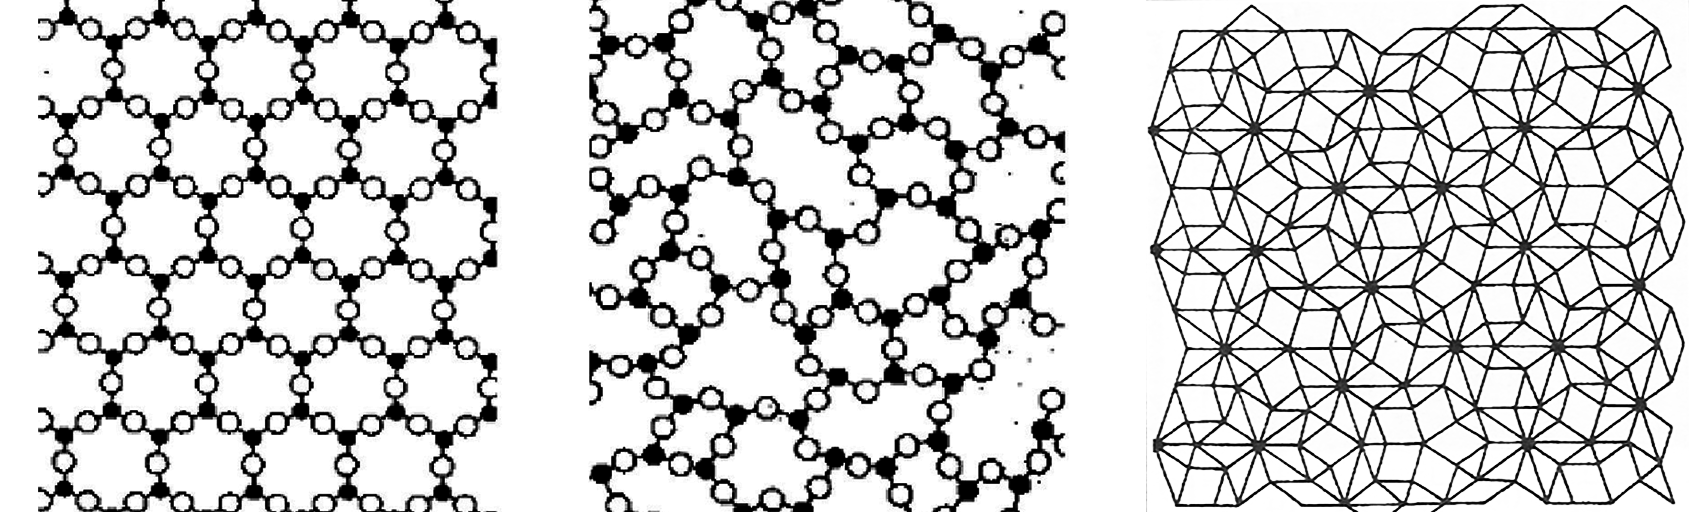
\includegraphics[width=\textwidth, keepaspectratio=true]{pic/1-01}
        \caption{晶体、非晶体与准晶体的粒子排列}
        \label{fig:1-01}
    \end{figure}

\subsection{晶格}
    晶体中,粒子排列的具体周期性结构称为\textbf{晶格}\index{晶格}。不同晶体具有不同的粒子排列结构,我们称为具有不同的晶格。
    
    我们在本节介绍若干种常见的晶体结构。为了便于理解,我们把晶格视为球体的堆积,即一个个原子呈球形,且彼此紧密的堆积在一起。

    \autoref{tab:1-1}引入下列晶格参数,从而方便地描述晶格特性:
    \begin{table}[!htbp]
        \centering
        \setlength{\tabcolsep}{1em}
        \begin{tabular}{lcl}
            \toprule
            晶格参数    &   字母表示    &   含义    \\
            \midrule
            晶格常数    &   $a$     &   标注某条棱的长度\\
            有效原子数  &           &   晶格内所含有的原子数\\
            配位数      &   $n$     &   与某原子距离最近的原子数\\
            最近邻距离  &           &   与某原子距离最近的原子的距离\\
            致密度      &   $\rho$  &   $\mbox{致密度}\rho=\frac{\mbox{有效原子数}\times \mbox{原子体积}}{\mbox{晶格体积}}$\\
            密排方向    &           &   在某个方向上原子密排\\
            \bottomrule
        \end{tabular}
        \caption{晶格常数}
        \label{tab:1-1}
    \end{table}

\newpage 
\subsubsection{第一类晶格:立方体结构}
    将同种粒子放在正方形的顶点上,即可得到平面的二位正方结构;\\
    同理我们推广到三维情况。所有的立方体结构晶格如\autoref{tab:1-2}所示。
    \begin{itemize}[itemsep=0pt,parsep=0pt]
        \item \textbf{简单立方}\index{简单立方}:将同种粒子放在立方体的顶点上,即为简单立方结构。\footnote{简单立方结构在自然界中极其罕见,目前唯一实例是钋($Po$)的$\alpha$相晶体}
        \item \textbf{面心立方}\index{面心立方}:在简单立方的基础上,若立方体每个面心还有一个粒子,即为面心立方结构。\footnote{应当指出,面心立方即为最密堆积的ABC结构。}
        \item \textbf{体心立方}\index{体心立方}:在简单立方的基础上,若立方体体心还有一个粒子,即为面心立方结构。
    \end{itemize}

    \begin{table}[!htbp]
        \centering
        \resizebox{\textwidth}{!}{
        \setlength{\tabcolsep}{1em}
        \begin{tabular}{ccccc}
                & 二维正方 & 简单立方 & 面心立方 & 体心立方\\
                & 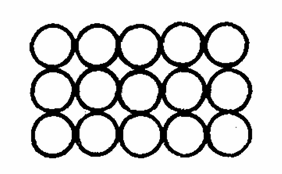
\includegraphics[height=6em, keepaspectratio=true]{pic/1-02} & 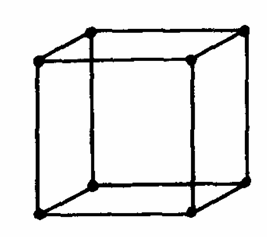
\includegraphics[height=6em, keepaspectratio=true]{pic/1-03} & 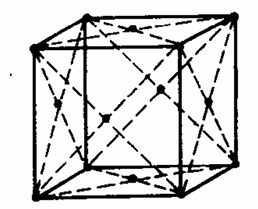
\includegraphics[height=6em, keepaspectratio=true]{pic/1-04} & 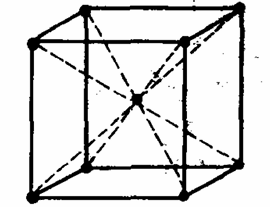
\includegraphics[height=6em, keepaspectratio=true]{pic/1-05}\\
            晶格常数$a$ & a & a & a & a \\
            密排方向    &沿边$a=2r$&沿棱$a=2r$&沿面对角线$\sqrt{2}a=4r$&沿体对角线$\sqrt{3}a=4r$\\
            有效原子数  &$4\times \frac{1}{4} = 1$&$8\times \frac{1}{8} = 1$&$8\times \frac{1}{8} + 6\times \frac{1}{2}= 4$&$8\times \frac{1}{8} + 1\times 1= 2$\\
            配位数$n$   &4&6&12&8\\
            最近邻距离  &$a$&$a$&$\frac{\sqrt{2}}{2}a$&$\frac{\sqrt{3}}{2}a$\\
            致密度$\rho$&&$\rho_1=\frac{1\times \frac{4}{3} \pi r^3}{(2r)^3} = \frac{\pi}{6}$&$\rho_2=\frac{4\times \frac{4}{3} \pi r^3}{(2\sqrt{2}r)^3} = \frac{\sqrt{2}}{6}\pi$&$\rho_3=\frac{2\times \frac{4}{3} \pi r^3}{(\frac{4}{\sqrt{3}}r)^3} = \frac{\sqrt{3}}{8}\pi$\\
        \end{tabular}
        }
        \caption{立方体结构晶格}
        \label{tab:1-2}
    \end{table}

\subsubsection{第二类晶格:密堆积结构}
    我们考虑这样的问题:如何排列,可以使得二维平面内可以放下最多的球体?这就是二维等径球最密堆积问题。可以证明,\autoref{fig:1-02}这样的排列是平面内的最密排列,称这种原子球在平面内最紧密排列的方式为\textbf{密排面}\index{密排面}。

    \begin{figure}[!htbp]
        \centering
        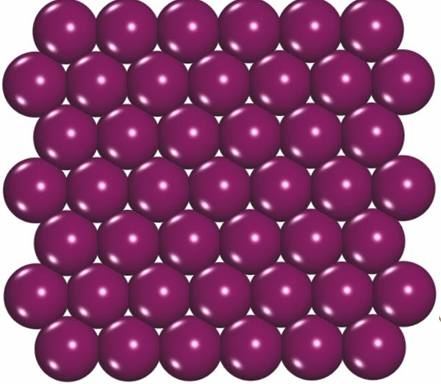
\includegraphics[height=8em, keepaspectratio=true]{pic/1-09}
        \caption{二维等径球最密堆积}
        \label{fig:1-02}
    \end{figure}

    仔细观察\autoref{fig:1-03}这样的密排面,我们应当注意到它具有两种不同的三角形空隙——一种三角形的尖尖朝上,如图中的第一排空隙B所示;另一种的三角形的尖尖朝下,如图中的第二排空隙C所示。两种空隙彼此交错。

    \begin{figure}[!htbp]
        \centering
        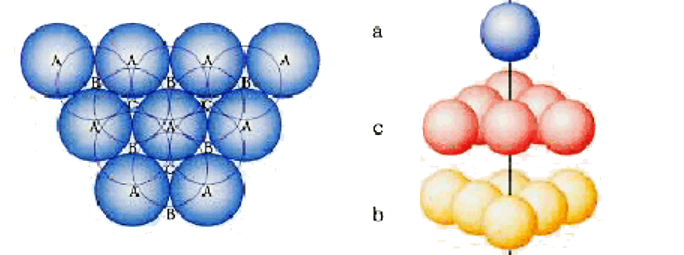
\includegraphics[height=8em, keepaspectratio=true]{pic/1-10}
        \caption{密排面的空隙}
        \label{fig:1-03}
    \end{figure}

    推广到三维情况,为了堆积得最紧密,由若干个这样的密排面一层层叠加起来,将一层的球心对准另一层的空隙。这就出现了两种堆叠方式:堆叠B空隙还是C空隙?并由此形成了两种完全不同密堆积结构:AB型,与ABC型,如\autoref{fig:1-04}所示。
    
    顾名思义,第一种堆积方式即第一层的球心A对齐第二层的空隙B,并继续堆积第三层的球心A';第二种堆积方式则是第一层的球心先对齐第二层的空隙B,再对齐第三层的另一种空隙C,最后堆积新的一层的球心。
    
    \begin{figure}[!htbp]
        \centering
        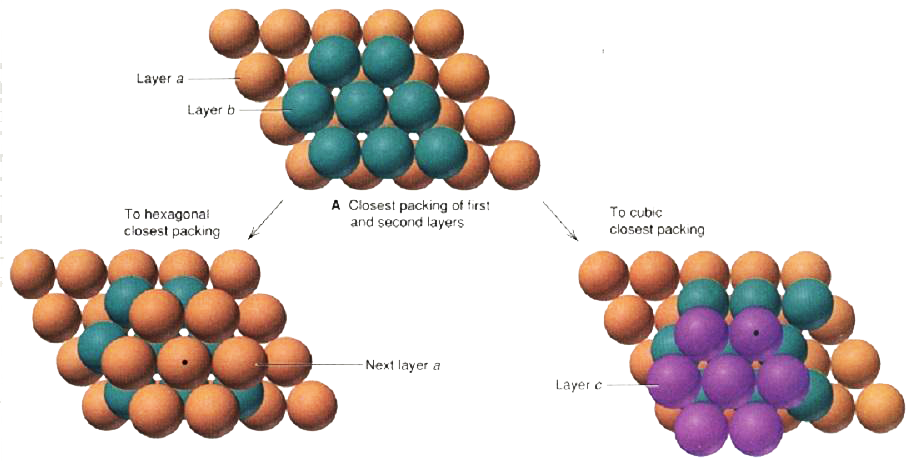
\includegraphics[height=14em, keepaspectratio=true]{pic/1-11}
        \caption{两种密堆积结构:AB型与ABC型}
        \label{fig:1-04}
    \end{figure}

    应当指出:ABC型堆积中,BC的顺序并不重要。根据观察的角度不同,空隙的指向也会变换,我们只要求BC两层空隙的角度相反。也可以认为,对于$\dots$\textcolor{red}{\textbf{ABC}}ABC$\dots$的堆积,我们从相反方向观察,就自然变成了$\dots$CB\textcolor{red}{\textbf{ACB}}A$\dots$的堆积。

    归纳密堆积结构晶格如\autoref{tab:1-3}所示:
    \begin{table}[!htbp]
        \centering
        \resizebox{\textwidth}{!}{
        \setlength{\tabcolsep}{1em}
        \begin{tabular}{cccc}
                & 二维六角 & 六角密排AB & 面心立方ABC\\
                & 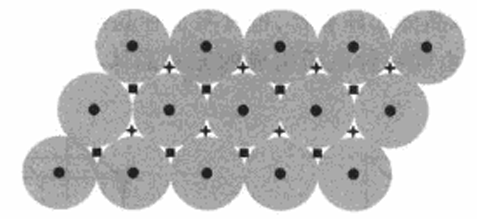
\includegraphics[height=4em, keepaspectratio=true]{pic/1-06} & 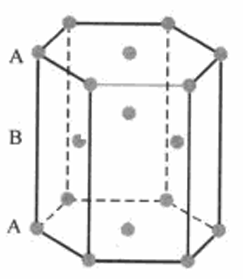
\includegraphics[height=6em, keepaspectratio=true]{pic/1-07} & 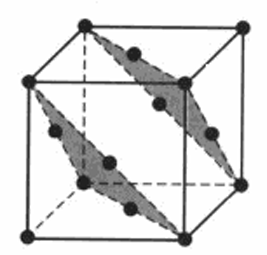
\includegraphics[height=6em, keepaspectratio=true]{pic/1-08}\\
            晶格常数$a$ & a & a \& c & a \\
            密排方向    &沿两近邻粒子方向$a=2r$&水平方向$a=2r$垂直方向$h=\frac{\sqrt{6}}{2}a=\frac{c}{2}$&沿面对角线$\sqrt{2}a=4r$\\
            有效原子数  &1&2&4\\
            配位数$n$   &6&12&12\\
            最近邻距离$a$&$a$&$a$&$\frac{\sqrt{2}}{2}a$\\
            致密度$\rho$&&$\rho_1=\frac{2\times \frac{4}{3} \pi r^3}{(\frac{\sqrt{3}}{4}a)^3 \times 2\times h} = \frac{\sqrt{2}}{6} \pi$&$\rho_2=\frac{4\times \frac{4}{3} \pi r^3}{(2\sqrt{2}r)^3} = \frac{\sqrt{2}}{6}\pi$\\
        \end{tabular}
        }
        \caption{密堆积结构晶格}
        \label{tab:1-3}
    \end{table}

    我们给出这样的两个要点:
    \begin{enumerate}[itemsep=0pt,parsep=0pt]
        \item \textbf{面心立方}既可以从立方体结构的角度考虑,而如果我们从立方体的体对角线看过去——这就是密堆积结构的ABC型。
        \item \textbf{面心立方}与\textbf{体心立方}互为倒格子。这将是\autoref{chap:2}的重要结论。
    \end{enumerate}

\subsubsection{第三类晶格:复式晶格}
    上述的第一类晶格与第二类晶格,常见于同一种原子所组成的单质晶体。我们现在介绍一些由多种原子或离子所组成的化合物晶体的晶格。






    
\section{晶体的平移对称性}
\section{晶体的方向性}
\section{晶体的宏观对称性}

\chapter{倒格子与波矢空间}\label{chap:2}
\section{倒格子}
\section{布里渊区}
\section{X射线衍射}

\chapter{晶格振动}
\section{一维单原子链的振动}
\section{一维双原子链的振动}
\section{三维晶格的振动}

\chapter{能带理论}
\section{自由电子近似}
\section{近自由电子近似}
\section{紧束缚近似}